\documentclass[conference]{IEEEtran}
\usepackage{graphics}
\usepackage{epsfig}
\usepackage{mathptmx}
\usepackage{times}
\usepackage{amsmath}
\usepackage{amssymb}
\usepackage{graphicx}
\usepackage{caption}
\usepackage{subcaption}
\usepackage{float}
\usepackage[flushmargin]{footmisc}

\begin{document}

\title{\LARGE \bf A GPU Block-Level Scheduling Method for Concurrent Kernels}

\author{\IEEEauthorblockN{Yidi Wang} \\
\IEEEauthorblockA{University of California, Riverside\\
yidi.wang@email.ucr.edu}
}

\maketitle

\begin{abstract}
Increasing amount of resources is available on current GPU, and concurrent kernel execution is allowed. However, the GPU resource usage is highly dependent on the submission order of kernels. In this project, an approach is proposed to reorder the concurrent kernels to reduce the total execution time and improve GPU resource utilization. 
\end{abstract}


\section{INTRODUCTION}
Nowadays, Graphics Processing Units (GPUs) are becoming more and more popular because of their outstanding and low-cost performance on parallelism compared to tranditional CPUs. The cost of rapid development of GPUs is that, the performance of GPUs are highly determined by some restrictions such as register file size, shared memory size, limit of threads number, etc. 

Users can make multiple kernels to run simultaneously by creating multiple streams and assigning different independent kernels onto those streams, in order to highly utilize the GPU resources and accelerate execution. The execution unit of a kernel is the thread block. Blocks are created during runtime and the number of blocks are defined by user when launching the kernel. The blocks are distributed to different Multiprocessors (SMs) to be processed. Whether a block can be assigned to a SM and start running is determined by the current available "spaces" of a SM. The limitations are number of threads and the size of shared memory per SM.

The default GPU scheduling policy is well illustrated in the prior work~\cite{c1}. The things to consider for a GPU scheduling policy should be different from CPU tasks scheduling. For example, Shortest Job First (SJF) is an optimal scheduling policy on CPU for minimum average waiting time (AWT). Because GPU resource limitations may stall the blocks in the kernel to run simultaneously, the optimal solution for CPU tasks may not work for GPU cases.

When a set of concurrent kernels are released, they are actually ordered in a FIFO queue. Because of the resource limitations, the hardware behaviors may differ when the kernels are reodered differently in the queue. 

Motivated by the above consideration and scenario, this project proposed a scheduling method for concurrent kernels. The method is based on the analysis of required resources of blocks. 
The contribution of the project are:
\begin{itemize}
   \item The proposed approach models the problem of deciding the submission order of a set of concurrent kernels as a growing 2D bin packing problem. The GPU resources are modeled to be the boundary of a rectangle bin, which can grow on the timeline. In this project, only the resource of number of threads per SM is considered.
   \item Shortest Job First (SJF) scheduling policy is implemented for GPU kernels. Naive approach, SJF approach and the proposed approach are compared in the evaluation part. The results are showed that the proposed approach can speedup execution while SJF is not to be optimum for GPU kernel scheduling.
\end{itemize}


\section{SYSTEMS WORK}

\subsection{Problem Simplification for Block-Level Scheduling}
The submission order of concurrent kernels are determined by the resources each block is going to consume. In order to simulate the block timelines, the maximum average number of blocks that will be assigned to each SM is considered. For example, a kernel has 16 blocks and the GPU has 15 SMs, then the number of blocks per SM is that $\frac{(16-1)}{15} + 1 = 2$.
\subsection{Dynamic Resource Mapping}
I created a rectangle to illustrate the resource usage. The y axis represent the number of used threads on one SM, and it has a ceiling of 2048 in the example as showed in Figure 2. The x axis represent the timeline. The rectangle is growable in this direction.  Each rectangle represent a chunk of resources in terms of the number of threads and time. Each time a block is fitted into the map, it will occupy one existing rectangle, and created two more rectangles. Iteratively, the blocks are fitted into the resource map from bottom to top, and left to right.
\subsection{Growing 2D Bin Packing}
At initialization, the kernels are sorted with block duration in descending order. Because of the features of the resource map mentioned above, a binary tree is used to store the represented resources of all the sub-rectangles. In the beginning, the size of the root rectangle is determined by the maximum number of threads one SM can accommodate by the execution time of the first block that is going to be fitted. Once a block is assigned, it will occupy the root of a subtree, and the two newly created rectangles are stored into its children. The left child represents the resources above the last assigned block, and the resource is dominant by only factor I considered in this project - the number of available threads on one SM. On the other hand, the right child represents the resources on the right of the block, and it can grow in the direction of time. Note thattThe left child will always be marked "ungrowable" since the current block can not have a longer duration than the previous ones. The situation that a space at the left of another block is found to be the best to grow will never happen, because if the algorithm let it grow, it may overlap with its right occupied spaces. The time complexity of the algorithm is $O(n^2)$.
\subsection{Greedy Choice}
Every time when a block is going to be assigned, the algorithm will search for a "best fit" empty space. If such a space with sufficient resources does not exist, then the algorithm will grow the rectangle that has sufficient resources and has the minimum start point.


\section{Baselines}
The experiments are run on GeForce GTX 1070, and the SDK version is CUDA 10.1. Every senario has an input json file, in which the number of kernels, kernel index, grid size, block size, duration and shared memory size are defined. In the experiments all the "shared memory" fields are set to be 0. The "duration", whose measuring unit is millisecond, can be approximated to be the execution time of each block. The block execution time is measured on the GPU using $globaltimer$ register. If the "duration" for each block is set to be 0, the actual block execution time is around 2us, which can be neglected compared to the set duration. When the kernel configurations, such as block size and grid size are changed, the actual block execution time will not change.

\subsection{Resource Limit}
The following limits are considered for GeForce GTX 1070:
\begin{itemize}
   \item Number of multiprocessors: : 15
   \item Maximum number of blocks per multiprocessor: 32
   \item Maximum number of threads per multiprocessor: 2048
   \item Maximum number of threads per block: 1024
\end{itemize}

\subsection{Single Kernel Scenarios}
In order to know whether each kernel is delayed by the others, I run a single kernel first. In the first, because the grid size equals to the number of SMs the GTX 1070 has, all 15 blocks can be assigned to SMs at launching, and they finishes at the same time. The execution time of each block equals to the execution time of this kernel. In the second scenario, the first 30 blocks are assigned to 15 SMs, and start running simultaneously. Due to the resource limitation, the last 15 blocks will wait until there are sufficient resources. The execution time of each block is as the same as what is gotten in the first scenario, but the kernel execution time doubles. \newline
\textit{Scenario 1}
\begin{itemize}
   \item Duration: 20ms
   \item Block size: 0 to 1024
   \item Grid size: 15
   \item Actual block running time: 20ms
   \item Actual kernelg running time: 20ms
\end{itemize}
\textit{Scenario 2}
\begin{itemize}
   \item Duration: $20ms$
   \item Block size: 0 to 1024
   \item Grid size: 45
   \item Actual block running time: 20ms
   \item Actual kernel running time: 40ms
\end{itemize}


\section{EVALUATION}
\subsection{Measurements}
Three metrics are used here to evaluate the performance the SJF policy and the proposed reordering policy: execution time, average response time (ART), and average waiting time (AWT). For the proposed policy, let's name it as "EE217".

\subsection{Block-level kernel scheduling}
\textit{Example.}
% TODO: 
Fig.\ref{fig:scenario1} depicts the block timeline produced by this experiment. Representaton $K_i:j$ means the $j$ th block of kernel $K_i$. As table\ref{table:scenario1_kernel} shows, three independent concurrent kernels, K1, K2, K3 were launched concurrently on different streams. For and simplification and symmetry, their durations are all set to be 20ms and grid size are all multiple of 15, so the same number of blocks of each kernel can be assigned to each SM evenly. If Naive Scheduling Policy (FIFO) was used, the launching order was default. The detailed block timeline on the first SM under FIFO and SJF is shown in Fig.\ref{fig:scenario1_naive}. At t = 0, the resources were sufficient, three blocks of K1 would be assigned to a SM, the remaining available number of threads on this SM was 512. Since one block of K2 requires 1024 threads, it could not start running at t = 0. At t = 20, all of the three blocks of k1 finished execution, then K2 could start running, and the number of available threads became 1024. Another four blocks of K3 can be also assigned. At t = 40, blocks which started running at t = 20 finished, then the last block of K3 could start. The blocks were divided into three groups to run, so the total running time was 3 times of a single block duration. The same behaviour was also oberved under SJF scheduling policy. From the kernel aspective, the timeline is shown as in Fig.\ref{fig:scenario1_kernel_naive}.

\begin{table}[h]
   \caption{Kernels used in scenario in Fig.\ref{fig:scenario1}}
   \centering
   \begin{tabular}{|c|c|c|c|}
   \hline
   \bf Kernels & \bf Grid size & \bf Block size & \bf Duration(ms)\\
   \hline
   K1 & 45 & 512 & 20 \\
   K2 & 15 & 1024 & 20\\ 
   K3 & 90 & 256 & 20 \\
   \hline
   \end{tabular}
   \label{table:scenario1_kernel}
\end{table}

The proposed scheduling policy, "EE217", reordered the kernels to maximize the resource utilization to reduce the execution time. The detailed block timeline on the first SM under FIFO and SJF is shown in Fig.\ref{fig:scenario1_opt}. Under this policy, at t = 0, the resources were sufficient, one block of K2 was assigned to a SM. The remaining available number of threads on this SM became 1024, which was also sufficient for two blocks of K1 to run simultaneously. At t = 20, all of the blocks which started at t = 0 finished. There were sufficient resources for all of the rest. The blocks were only divided into two groups, so the total running time was double of a single block duration. From the kernel aspective, the timeline is shown as in Fig.\ref{fig:scenario1_kernel_opt}.

 The results listed in table\ref{table:scenario1_result} show that SJF on GPU may not give an optimal average response time. The execution time is dependent on the kernel submission order to the hardware, and it can be reduced if they are reordered properly. In this case, a $100\%$ utilization and a 1.5 times speedup can be achieved by the proposed menthod.\par



\begin{table*}[h]
   \caption{Kernels used in scenario in Fig.\ref{fig:scenario1}}
   \centering
   \begin{tabular}{|c|c|c|c|c|c|}
   \hline
   \bf Policy & \bf Execution time(ms)& \bf ART(ms) & \bf AWT(ms) & \bf Speedup & \bf Utilization \\
   \hline
   FIFO & 60 & 40 & 13.33 & 1x & 66.67$\%$ \\
   SJF & 60 & 40 & 13.33 & 1x & 66.67$\%$\\ 
   EE217 & 40 & 20 & 6.67 & 1.5x & 100$\%$\\
   \hline
   \end{tabular}
   \label{table:scenario1_result}
\end{table*}

\begin{figure*}[!ht]
   \centering
   \begin{subfigure}{0.48\textwidth}
      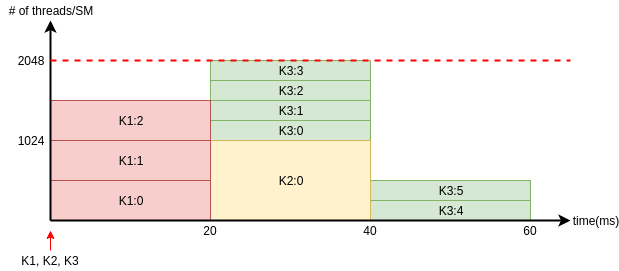
\includegraphics[width=\textwidth, height=120pt]{figs/scenario1_naive.png}
      \caption{Block timeline of naive and SJF}
      \label{fig:scenario1_naive}
   \end{subfigure}
   \begin{subfigure}{0.48\textwidth}
      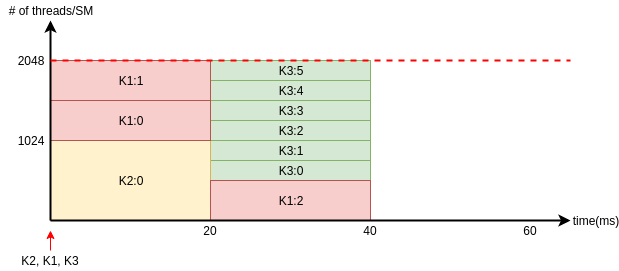
\includegraphics[width=\textwidth, height=120pt]{figs/scenario1_opt.png}
      \caption{Block timeline of optimum}
      \label{fig:scenario1_opt}
   \end{subfigure}
   \begin{subfigure}{0.48\textwidth}
      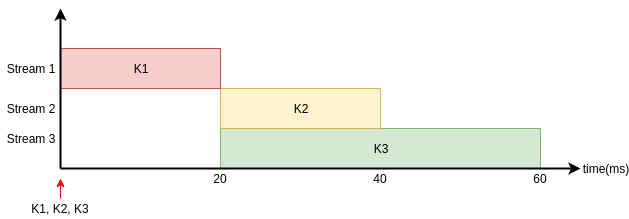
\includegraphics[width=\textwidth, height=90pt]{figs/scenario1_kernel_naive.png}
      \caption{Block timeline of optimum}
      \label{fig:scenario1_kernel_naive}
  \end{subfigure}
   \begin{subfigure}{0.48\textwidth}
      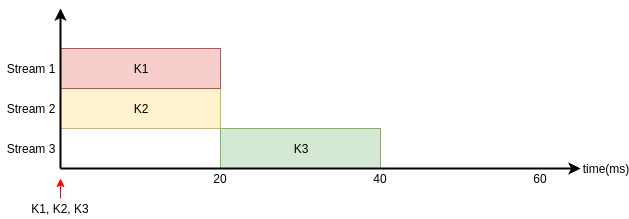
\includegraphics[width=\textwidth, height=90pt]{figs/scenario1_kernel_opt.png}
      \caption{Block timeline of optimum}
      \label{fig:scenario1_kernel_opt}
   \end{subfigure}
   \caption{Block timeline in scenario 1 on one SM}
   \label{fig:scenario1}
\end{figure*}

\textit{Example.}
In this example, I tested the scheduling policy with a set of randomly customized concurrent kernels. Figure depicts the block timeline produced by this experiment. As table\ref{table:scenario2_kernel} shows, ten independent concurrent kernels, K1 to K10 were launched concurrently on different streams. In order to fully test the proposed scheduling policy, the block size and grid size are also randomly given to the kernels. Under the naive policy, kernel launching order were default to be K1, K2, K3, K4, K5, K6, K7, K8, K9, K10. Under the SJF policy, the kernel launching order was K3, K5, K1, K8, K9, K4, K6, K10, K2, K7. Under the "EE217" policy, the kernel launching order was K7, K2, K6, K8, K10, K9, K3, K5, K4, K1. The results are listed in table \ref{table:scenario2_result}, in this case, the performance of SJF is the worst among three policies. Like in the previous scenario, the proposed policy increases utilization and speedup execution.\par

\begin{table}[h]
   \caption{Kernels used in scenario in Fig. } % title of Table
   \centering
   \begin{tabular}{|c|c|c|c|}
   \hline
   \bf Kernels & \bf Grid size & \bf Block size & \bf Duration(ms)\\
   \hline
   K1 & 48 & 512 & 20 \\
   K2 & 3 & 256 & 50\\ 
   K3 & 17 & 256 & 10 \\
   K4 & 15 & 1024 & 35 \\
   K5 & 23 & 128 & 15 \\ 
   K6 & 10 & 512 & 40 \\
   K7 & 1 & 1024 & 80 \\
   K8 & 30 & 256 & 20\\ 
   K9 & 12 & 128 & 25 \\
   K10 & 47 & 512 & 40 \\
   \hline
   \end{tabular}
   \label{table:scenario2_kernel}
\end{table}

\begin{table*}[h]
   \caption{Kernels used in scenario of random kernels} % title of Table
   \centering
   \begin{tabular}{|c|c|c|c|c|c|}
   \hline
   \bf Policy & \bf Execution time(ms)& \bf ART(ms) & \bf AWT(ms) & \bf Speedup & \bf Utilization \\
   \hline
   FIFO & 115 & 57.5 & 22 & 1x & 74.7$\%$ \\
   SJF & 155 & 25.5 & 25.5 & 0.74x & 55.42$\%$ \\ 
   EE217 & 95 & 60 & 19.5 & 1.21x & 90.43$\%$ \\
   \hline
   \end{tabular}
   \label{table:scenario2_result}
\end{table*}

\subsection{Experiment on shared memory}
Experiments with some shared memory are also done. As listed in table.\ref{table:shmem_kernel}, a series of same kernels were launched, but the execution time is difficult to be predicted. The running results are shown in Fig. which show that:
\begin{itemize}
   \item Fig.\ref{fig:shmem_case3} shows that execution time of independent blocks are increased due to shared memory access.
   \item Fig.\ref{fig:shmem_case4} shows that number of blocks that can run together on the same SM is limited due to the shared memory limit.
\end{itemize}

\begin{table*}[h]
   \caption{Kernels used in scenario in Fig.\ref{fig:shmem}}
   \centering
   \begin{tabular}{|c|c|c|c|c|c|}
   \hline
    & \bf Kernel number & \bf grid size & \bf block size & \bf shared memory size(KB) \\
    \hline
   Case 1 & 1 & 15 & 32 & 1024   \\
   Case 2 & 3 & 15 & 32 & 1024  \\ 
   Case 3 & 1 & 15 & 32 & 16384  \\
   Case 4 & 7 & 15 & 32 & 16384  \\
   \hline
   \end{tabular}
   \label{table:shmem_kernel}
\end{table*}

\begin{figure*}[h]
   \centering
   \begin{subfigure}{0.4\textwidth}
      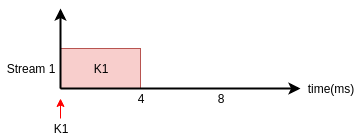
\includegraphics[width=\textwidth, height=60pt]{figs/shmem_1024_baseline.png}
      \caption{Case 1}
      \label{fig:shmem_case1}
   \end{subfigure}
   \begin{subfigure}{0.4\textwidth}
      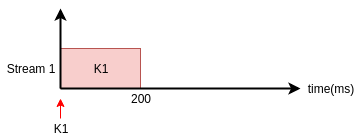
\includegraphics[width=\textwidth, height=60pt]{figs/shmem_16384_baseline.png}
      \caption{Case 3}
      \label{fig:shmem_case3}
   \end{subfigure}
   \begin{subfigure}{0.38\textwidth}
      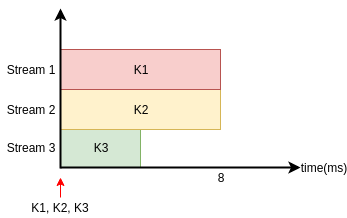
\includegraphics[width=\textwidth, height=80pt]{figs/shmem_1024.png}
      \caption{Case 2}
      \label{fig:shmem_case2}
  \end{subfigure}
   \begin{subfigure}{0.48\textwidth}
      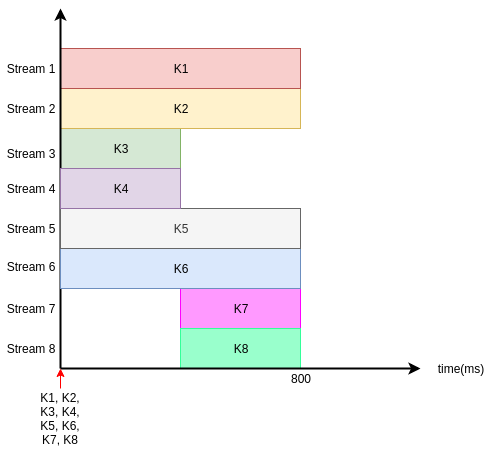
\includegraphics[width=\textwidth, height=120pt]{figs/shmem_16384.png}
      \caption{Case 4}
      \label{fig:shmem_case4}
   \end{subfigure}
   \caption{Timeline with shared memory on one SM}
   \label{fig:shmem}
\end{figure*}



\section{CONCLUSIONS}
With the support for parallelism, GPUs can utilize the resources more efficiently with a higher processing speed. As the observation shows in my work, the hardware decision and behaviors depends on the submission order of kernels. This project shows that a scheduling policy that reorders the kernels based on the analysis of kernel blocks is feasible. With this scheduling policy, I have successfully accelerated concurrent kernel execution and increase GPU resource utilizations compared to the naive kernel submission order and SJF. Also, I show that there is additional performance interference due to contention on shared memory.

\section*{APPENDIX}
Remember to change the line 13 in "multikernel.cuh" according to the number of SMs of your GPU.

\textbf{Json files.}
"example1.json" gives the example described in scenario 1. "example4.json" gives the example described in scenario 2. 
\footnote{More examples and usage can be found at:\\ \url{https://github.com/yidiwang21/ee217}}

\textbf{How to get the kernel submisssion order.}
If you only want to get the submission order of the input concurrent kernels, try: 
\begin{itemize}
   \item make
   \item ./exe [json file] [policy(0:naive, 1:sjf,  2:optimum)]
\end{itemize}

\textbf{How to draw block timeline.} Block timelines are drawn for each SM. Your will get the simulations for all the SMs by:
\begin{itemize}
   \item make
   \item sh run.sh -i [file] -s [policy(0:naive, 1:sjf, 2:optimum]
\end{itemize}

In Fig.\ref{fig:example_out}, an example of output timeline for one SM is given. This is the block timeline of scenario 1 under proposed policy.
\begin{figure}[h]
   \centering
   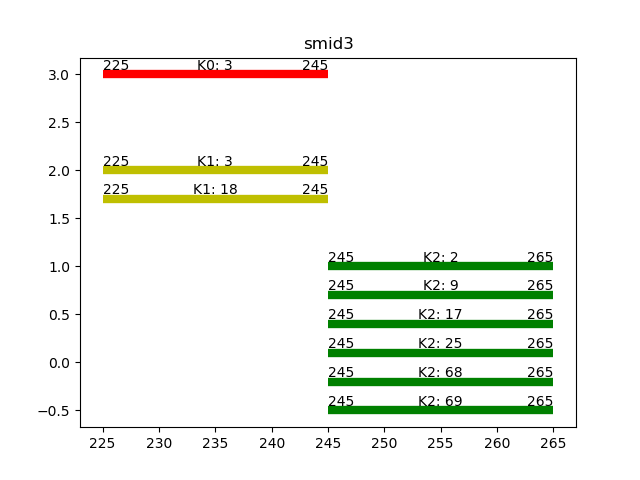
\includegraphics[width=0.48\textwidth, height=190pt]{figs/example1_opt.png}
   \caption{Example output timeline for one SM}
   \label{fig:example_out}
\end{figure}


\begin{thebibliography}{99}
\bibitem{c1} Tanya Amert, Nathan Otterness, Ming Yang, James H. Anderson, and F. Donelson Smith \emph{GPU Scheduling on the NVIDIA TX2: Hidden Details Revealed} (IEEE RTSS, 2017, Paris, France)
\end{thebibliography}

\end{document}